% Options for packages loaded elsewhere
\PassOptionsToPackage{unicode}{hyperref}
\PassOptionsToPackage{hyphens}{url}
%
\documentclass[
  twocolumn]{article}
\usepackage{lmodern}
\usepackage{amsmath}
\usepackage{ifxetex,ifluatex}
\ifnum 0\ifxetex 1\fi\ifluatex 1\fi=0 % if pdftex
  \usepackage[T1]{fontenc}
  \usepackage[utf8]{inputenc}
  \usepackage{textcomp} % provide euro and other symbols
  \usepackage{amssymb}
\else % if luatex or xetex
  \usepackage{unicode-math}
  \defaultfontfeatures{Scale=MatchLowercase}
  \defaultfontfeatures[\rmfamily]{Ligatures=TeX,Scale=1}
\fi
% Use upquote if available, for straight quotes in verbatim environments
\IfFileExists{upquote.sty}{\usepackage{upquote}}{}
\IfFileExists{microtype.sty}{% use microtype if available
  \usepackage[]{microtype}
  \UseMicrotypeSet[protrusion]{basicmath} % disable protrusion for tt fonts
}{}
\makeatletter
\@ifundefined{KOMAClassName}{% if non-KOMA class
  \IfFileExists{parskip.sty}{%
    \usepackage{parskip}
  }{% else
    \setlength{\parindent}{0pt}
    \setlength{\parskip}{6pt plus 2pt minus 1pt}}
}{% if KOMA class
  \KOMAoptions{parskip=half}}
\makeatother
\usepackage{xcolor}
\IfFileExists{xurl.sty}{\usepackage{xurl}}{} % add URL line breaks if available
\IfFileExists{bookmark.sty}{\usepackage{bookmark}}{\usepackage{hyperref}}
\hypersetup{
  pdftitle={2 Column Rmarkdown template},
  pdfauthor={Me\textbackslash dagger,\textbackslash S, Her\textbackslash ddagger, Him\textbackslash dagger, Them\textbackslash ddagger},
  hidelinks,
  pdfcreator={LaTeX via pandoc}}
\urlstyle{same} % disable monospaced font for URLs
\usepackage[margin=1.5cm]{geometry}
\usepackage{graphicx}
\makeatletter
\def\maxwidth{\ifdim\Gin@nat@width>\linewidth\linewidth\else\Gin@nat@width\fi}
\def\maxheight{\ifdim\Gin@nat@height>\textheight\textheight\else\Gin@nat@height\fi}
\makeatother
% Scale images if necessary, so that they will not overflow the page
% margins by default, and it is still possible to overwrite the defaults
% using explicit options in \includegraphics[width, height, ...]{}
\setkeys{Gin}{width=\maxwidth,height=\maxheight,keepaspectratio}
% Set default figure placement to htbp
\makeatletter
\def\fps@figure{htbp}
\makeatother
\setlength{\emergencystretch}{3em} % prevent overfull lines
\providecommand{\tightlist}{%
  \setlength{\itemsep}{0pt}\setlength{\parskip}{0pt}}
\setcounter{secnumdepth}{-\maxdimen} % remove section numbering
\usepackage{wrapfig}
\usepackage{lipsum}
\newcommand{\bcenter}{\begin{center}}
\newcommand{\ecenter}{\end{center}}
\usepackage{caption}
\usepackage{xcolor}
\ifluatex
  \usepackage{selnolig}  % disable illegal ligatures
\fi
\newlength{\cslhangindent}
\setlength{\cslhangindent}{1.5em}
\newlength{\csllabelwidth}
\setlength{\csllabelwidth}{3em}
\newenvironment{CSLReferences}[2] % #1 hanging-ident, #2 entry spacing
 {% don't indent paragraphs
  \setlength{\parindent}{0pt}
  % turn on hanging indent if param 1 is 1
  \ifodd #1 \everypar{\setlength{\hangindent}{\cslhangindent}}\ignorespaces\fi
  % set entry spacing
  \ifnum #2 > 0
  \setlength{\parskip}{#2\baselineskip}
  \fi
 }%
 {}
\usepackage{calc}
\newcommand{\CSLBlock}[1]{#1\hfill\break}
\newcommand{\CSLLeftMargin}[1]{\parbox[t]{\csllabelwidth}{#1}}
\newcommand{\CSLRightInline}[1]{\parbox[t]{\linewidth - \csllabelwidth}{#1}\break}
\newcommand{\CSLIndent}[1]{\hspace{\cslhangindent}#1}

\title{2 Column Rmarkdown template}
\author{Me\textsuperscript{\(\dagger\),\(\S\)},
Her\textsuperscript{\(\ddagger\)}, Him\textsuperscript{\(\dagger\)},
Them\textsuperscript{\(\ddagger\)}}
\date{}

\begin{document}
\maketitle
\begin{abstract}
Here you can add a bunch of text for your abstract, it will be formatted
independently from the rest of the document, so you can't use as many of
the tricks you'd use in markdown, but you can write in \textit{italics},
\textbf{bold} and \textcolor{red}{different} \textcolor{blue}{colors}.
\end{abstract}

\hypertarget{section-title}{%
\subsection{Section Title}\label{section-title}}

Here is some text, you can type as you would in any other program, in
this case we've set up the formatting to make this 2-lines. You can add
citations(Brahmi and Gall 2006) by searching Pubmed for example using
the embedded tools in Rstudio. The code above makes it so you can do
custom aligning of figures.

The great thing about Rmd writing is you can include R code inline,
which will keep things up to date when your data or other things change.
For example, if you've `knitted' this document today, then the date is
Thu Jan 7 17:48:10 2021.

Other things you can do might involve more complicated code in a code
chunk like a plot. For example:

\begin{figure}
\centering
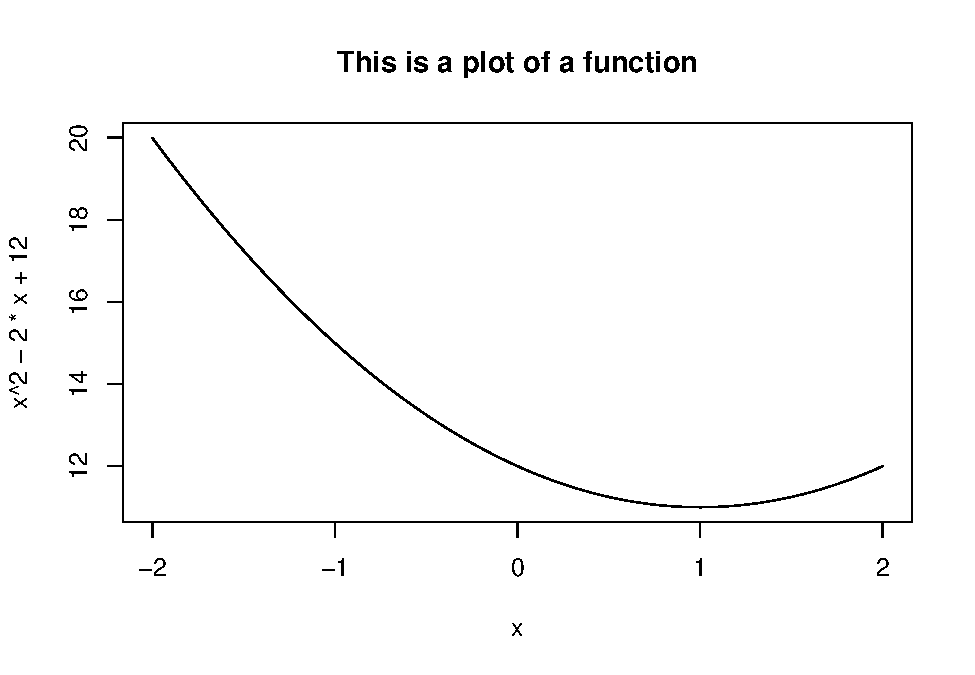
\includegraphics{2_Col_template_files/figure-latex/unnamed-chunk-1-1.pdf}
\caption{Here we can write the caption for the figure, for super long
captions you might not want to use this approach}
\end{figure}

Other words, Other words, Other words, Other words, Other words, Other
words, Other words, Other words, Other words, Other words, Other words,
Other words, Other words, Other words, Other words, Other words, Other
words, Other words, Other words, Other words, Other words, Other words,
Other words, Other words, Other words, Other words, Other words, Other
words, Other words, Other words, Other words, Other words, Other words,
Other words, Other words, Other words, Other words, Other words, Other
words, Other words, Other words, Other words, Other words, Other words,
Other words, Other words, Other words, Other words, Other words, Other
words, Other words, Other words, Other words, Other words, Other words,
Other words, Other words, Other words, Other words, Other words, Other
words, Other words, Other words, Other words, Other words, Other words,
Other words, Other words, Other words, Other words, Other words, Other
words, Other words, Other words, Other words, Other words, Other words,
Other words, Other words, Other words, Other words, Other words, Other
words, Other words, Other words, Other words, Other words, Other words,
Other words, Other words, Other words, Other words, Other words, Other
words, Other words, Other words, Other words, Other words, Other words,
Other words, Other words, Other words, Other words, Other words, Other
words, Other words, Other words, Other words.

\hypertarget{another-section-title}{%
\subsection{Another Section title}\label{another-section-title}}

Here, maybe you want to pull in some example data and run a plot on it.
We can run some code in the background, save the data to a folder, then
load it back in to plot:

\begin{figure}
\centering
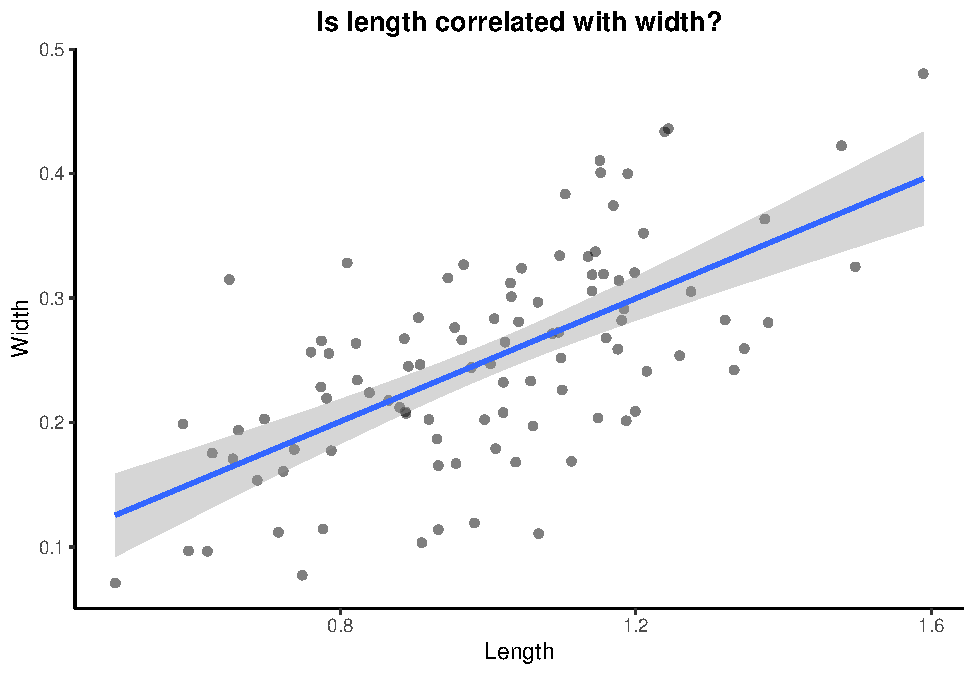
\includegraphics{2_Col_template_files/figure-latex/unnamed-chunk-2-1.pdf}
\caption{This is the caption, here you can see the length and width are
correlated, but noisy}
\end{figure}

So maybe we concluded that the effect was real but maybe a bit weak. And
then we blathered about it for a while\ldots. blather, blather, blather,
blather, blather, blather, blather, blather, blather, blather, blather,
blather, blather, blather, blather, blather, blather, blather, blather,
blather, blather, blather, blather, blather, blather, blather, blather,
blather, blather, blather, blather, blather, blather, blather, blather,
blather, blather, blather, blather, blather, blather, blather, blather,
blather, blather, blather, blather, blather, blather, blather, blather,
blather, blather, blather, blather, blather, blather, blather, blather,
blather, blather, blather, blather, blather, blather, blather, blather,
blather, blather, blather.

\hypertarget{but-is-there-another-factor-involved}{%
\subsection{But is there another factor
involved?}\label{but-is-there-another-factor-involved}}

So we realized that some of our animals were 1 day old and some were 4
days old, could this have any effect on the length vs.~width that we
previously analyzed? Luckily we saved the simulated data and can load it
back in, this time considering \texttt{Age}.

\begin{figure}
\centering
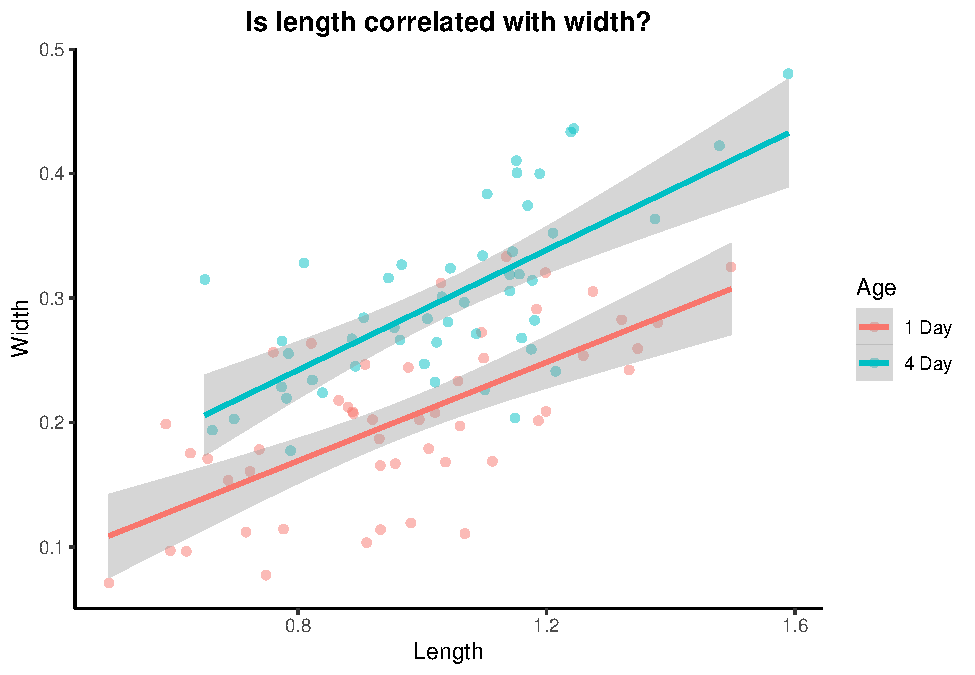
\includegraphics{2_Col_template_files/figure-latex/unnamed-chunk-3-1.pdf}
\caption{Now when we look at age, it has a clear effect}
\end{figure}

So that's it.

\hypertarget{refs}{}
\begin{CSLReferences}{1}{0}
\leavevmode\hypertarget{ref-Brahmi2006}{}%
Brahmi, Frances A., and Carole Gall. 2006. {``EndNote® and Reference
Manager® Citation Formats Compared to {``}Instructions to Authors{''} in
Top Medical Journals.''} \emph{Medical Reference Services Quarterly} 25
(2): 49--57. \url{https://doi.org/10.1300/j115v25n02_04}.

\end{CSLReferences}

\end{document}
